\chapter{Исследовательский раздел}

\section{Технические характеристики}

Технические характеристики устройства, на котором запускалась программа:

\begin{enumerate}
	\item операционная система Ubuntu, 22.04.4~\cite{ubuntu} c версией ядра 5.19.17~\cite{};
	\item память 16 Гайт;
	\item процессор 2,5 ГГц 4‑дерный процессор Intel Core i5-10300H~\cite{intel}.
\end{enumerate}

\section{Исследование работы программы}

Для исследования работы была разработаны вспомогательные программы:
\begin{enumerate}
	\item программа, которая создает неименованный программный канал для передачи сообщение созданным процессам--потомкам;
	\item программа, которая создает обработчик и послыает сигнал созданному процессу--потомку;
	\item программа читатели--писатели.
\end{enumerate}

На рисунке~\ref{img:exmaple-general} продемонстрирована работа загружамого модуля при чтении файла general.

\begin{figure}[h]
	\centering
	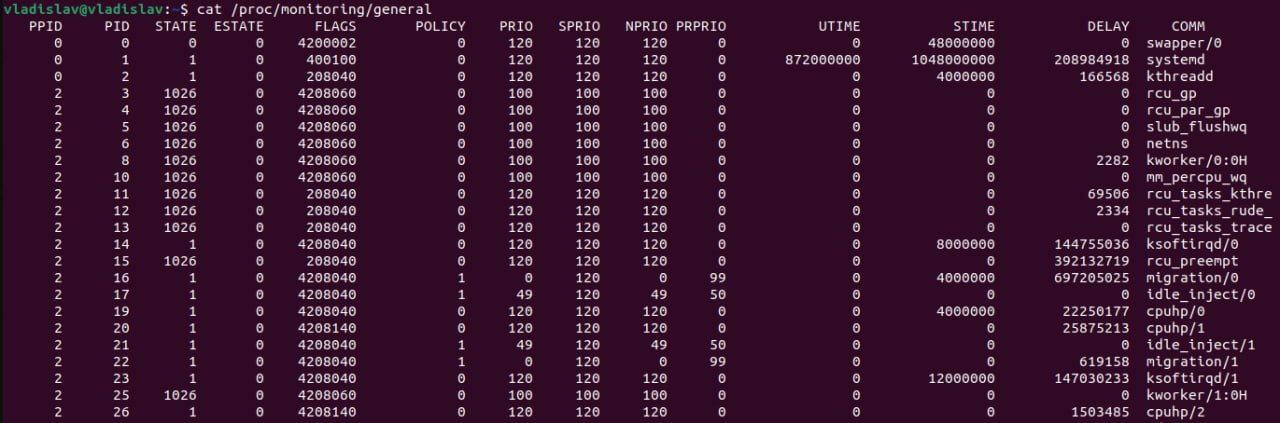
\includegraphics[width=0.9\textwidth]{img/example-general}
	\caption{Демонстрация работы программы при чтении из файла \texttt{general}}
	\label{img:exmaple-general}
\end{figure}


\begin{figure}[h]
	\centering
	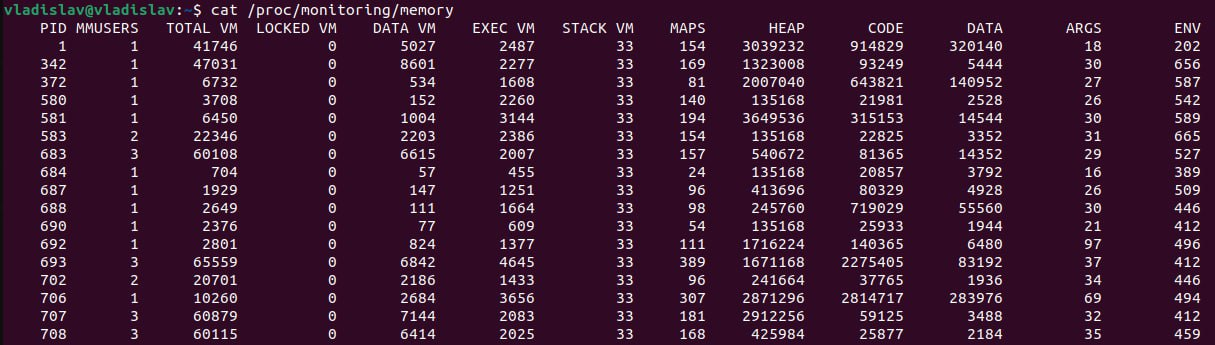
\includegraphics[width=0.9\textwidth]{img/example-memory}
	\caption{Демонстрация работы программы при чтении из файла \texttt{memory}}
	\label{img:exmaple-memory}
\end{figure}

\begin{figure}[h]
	\centering
	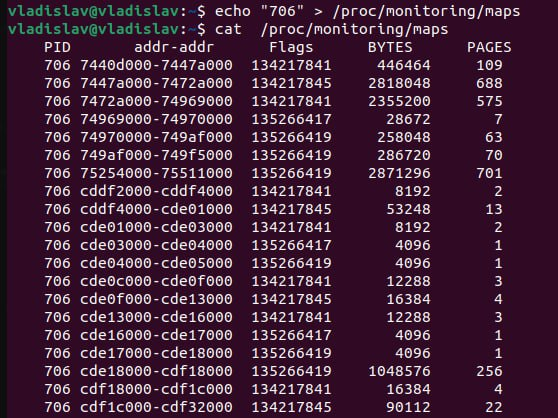
\includegraphics[width=0.7\textwidth]{img/example-maps}
	\caption{Демонстрация работы программы при записи в файл и чтении из файла \texttt{maps}}
	\label{img:exmaple-maps}
\end{figure}

\begin{figure}[h]
	\centering
	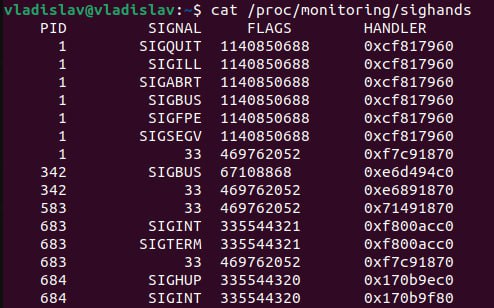
\includegraphics[width=0.7\textwidth]{img/example-sighand}
	\caption{Демонстрация работы программы при записи в файл и чтении из файла \texttt{sighands}}
	\label{img:exmaple-sighand}
\end{figure}
